% Method overview (camera-ready), drawn at print size. Build:  pdflatex pipeline.tex
% Panel 2 describes the program that produced the reported results: runs/evolve_run7_multi/candidates/run7_best_gen035_0.5888.py
\documentclass[border=2pt]{standalone}
\usepackage[T1]{fontenc}
\usepackage{helvet}
\renewcommand{\familydefault}{\sfdefault}
\usepackage{tikz}
\usetikzlibrary{arrows.meta,positioning,fit,backgrounds,calc}
\definecolor{cInk}{HTML}{0b0b0b}
\definecolor{cMuted}{HTML}{52514e}
\definecolor{cLine}{HTML}{8a8a86}
\definecolor{cBlue}{HTML}{2a78d6}
\definecolor{cBlueBg}{HTML}{E9F1FB}
\definecolor{cGrayBg}{HTML}{F1F0EC}
\newcommand{\hd}[1]{{\fontsize{7.5}{8.4}\selectfont\bfseries #1}}
\newcommand{\hdn}[1]{{\fontsize{7.5}{8.4}\selectfont #1}}
\newcommand{\ds}[1]{{\color{cMuted}#1}}
\begin{document}
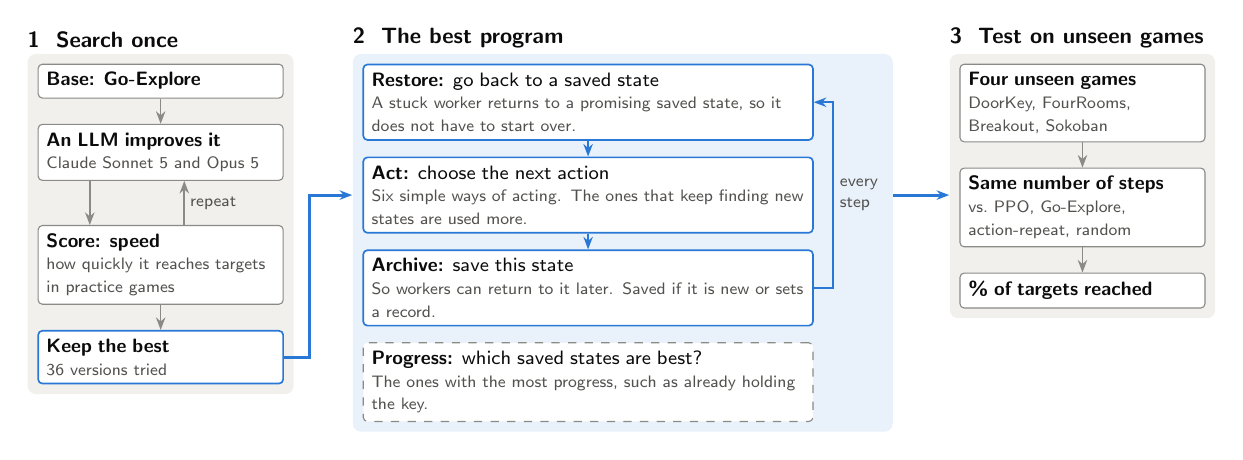
\begin{tikzpicture}[
  >={Stealth[length=1.6mm]},
  box/.style={rounded corners=1.5pt, draw=cLine, fill=white, line width=0.4pt, inner sep=3pt, align=left, text=cInk, text width=#1, font={\fontsize{6.5}{8.2}\selectfont\hyphenpenalty 10000 \exhyphenpenalty 10000 }},
  hook/.style={rounded corners=1.5pt, draw=cBlue, fill=white, line width=0.6pt, inner sep=3pt, align=left, text=cInk, text width=#1, font={\fontsize{6.5}{8.2}\selectfont\hyphenpenalty 10000 \exhyphenpenalty 10000 }},
  ttl/.style={font=\fontsize{8}{9.5}\selectfont\bfseries, text=cInk, anchor=south west, inner sep=0pt},
  sub/.style={font=\fontsize{6.5}{7.5}\selectfont, text=cMuted},
  flow/.style={->, line width=0.6pt, draw=cLine},
]
% ------------------------------------------------------------------ 1. search
\node[box=29mm] (seed) {\hd{Base: Go-Explore}};
\node[box=29mm, below=3.2mm of seed] (llm) {\hd{An LLM improves it}\\\ds{Claude Sonnet~5 and Opus~5}};
\node[box=29mm, below=5.6mm of llm] (fit) {\hd{Score: speed}\\\ds{how quickly it reaches targets in practice games}};
\node[box=29mm, below=3.2mm of fit, draw=cBlue, line width=0.6pt] (best) {\hd{Keep the best}\\\ds{36 versions tried}};
\draw[flow] (seed) -- (llm);
\draw[flow] ([xshift=-9mm]llm.south) -- ([xshift=-9mm]fit.north);
\draw[flow] ([xshift=3mm]fit.north) -- node[right, sub, xshift=-1.5pt] {repeat} ([xshift=3mm]llm.south);
\draw[flow] (fit) -- (best);

% ------------------------------------------------------------------ 2. the best program
\node[hook=55mm, right=10mm of seed.north east, anchor=north west] (res) {\hd{Restore:}\hdn{ go back to a saved state}\\
  \ds{A stuck worker returns to a promising saved state, so it does not have to start over.}};
\node[hook=55mm, below=2mm of res] (act) {\hd{Act:}\hdn{ choose the next action}\\
  \ds{Six simple ways of acting. The ones that keep finding new states are used more.}};
\node[hook=55mm, below=2mm of act] (arc) {\hd{Archive:}\hdn{ save this state}\\
  \ds{So workers can return to it later. Saved if it is new or sets a record.}};
\node[box=55mm, below=2mm of arc, dashed] (det) {\hd{Progress:}\hdn{ which saved states are best?}\\
  \ds{The ones with the most progress, such as already holding the key.}};
\draw[flow, draw=cBlue] (res) -- (act);
\draw[flow, draw=cBlue] (act) -- (arc);
\draw[flow, draw=cBlue] (arc.east) -- ++(2.4mm,0) |- node[pos=0.25, right, sub, align=left, xshift=-1pt] {every\\step} (res.east);
\coordinate (padr) at ($(arc.east)+(8.8mm,0)$);

% ------------------------------------------------------------------ 3. test
\node[box=29mm, right=18.5mm of res.north east, anchor=north west] (tasks) {\hd{Four unseen games}\\\ds{DoorKey, FourRooms, Breakout, Sokoban}};
\node[box=29mm, below=3.2mm of tasks] (vs) {\hd{Same number of steps}\\\ds{vs.\ PPO, Go-Explore, action-repeat, random}};
\node[box=29mm, below=3.2mm of vs] (out) {\hd{\% of targets reached}};
\draw[flow] (tasks) -- (vs);
\draw[flow] (vs) -- (out);

% ------------------------------------------------------------------ backdrops, titles, stage arrows
\begin{scope}[on background layer]
  \node[fill=cGrayBg, rounded corners=3pt, fit=(seed)(llm)(fit)(best), inner sep=3.5pt] (b1) {};
  \node[fill=cBlueBg, rounded corners=3pt, fit=(res)(act)(arc)(det)(padr), inner sep=3.5pt] (b2) {};
  \node[fill=cGrayBg, rounded corners=3pt, fit=(tasks)(vs)(out), inner sep=3.5pt] (b3) {};
\end{scope}
\node[ttl] at ([yshift=2pt]b1.north west) {1\ \ Search once};
\node[ttl] at ([yshift=2pt]b2.north west) {2\ \ The best program};
\node[ttl] at ([yshift=2pt]b3.north west) {3\ \ Test on unseen games};
\draw[->, line width=1.1pt, draw=cBlue] (best.east) -- ++(3.2mm,0) |- (b2.west |- act);
\draw[->, line width=1.1pt, draw=cBlue] (b2.east |- act) -- (b3.west |- act);
\end{tikzpicture}
\end{document}
